\documentclass{article}

% Packages for setting up page margins
\usepackage[margin=1in]{geometry}

\usepackage{graphicx, setspace, amsmath, mathtools, amssymb, url, float}
\setlength{\parskip}{2mm}
\graphicspath{ {./images/} }

% Title
\title{CS535 Design and Analysis of Algorithms - Assignment 1}
\author{Batkhishig Dulamsurankhor - A20543498}
\date{\today} % Use \date{} for no date

\begin{document}

\maketitle

\begin{enumerate}
  \item 0xDA0121C8=(13*16+10).(0*16+1).(2*16+1).(12*16+8)=218.1.33.200

  First byte is 0xDA=11011010, because it starts with 110, it is Class C.
  \item
    \begin{enumerate}
      \item 36th block of class A: 255.

      Class A range: 0.0.0.0 to 127.255.255.255. Each block consists of $2^{24}$ addresses.

      36th block: 35.0.0.0 to 35.255.255.255.

      \item 12th block of class B

      Class B range: 128.0.0.0 to 191.255.255.255. Each block consists of $2^{16}$ addresses.

      12th block: 128.15.0.0 to 128.15.255.255.
      \item 318th block of class B

      Class B range: 128.0.0.0 to 191.255.255.255. Each block consists of $2^{16}$ addresses.

      318th block: 129.63.0.0 to 129.63.255.255.
      \item 3rd block of class C

      Class B range: 192.0.0.0 to 223.255.255.255. Each block consists of $2^{8}$ addresses.

      3rd block: 192.0.3.0 to 192.0.3.255.
    \end{enumerate}
  \item Assume classful addressing. If one of the hosts in a certain network has an IP address 129.6.0.10 (4 points)
  \begin{enumerate}
    \item What is the network address? (1 point)
    
    129=10000001. So this is class B. The default mask is 255.255.0.0 and network address is 129.6.0.0.
    \item What are the netid and hostid of this host? (1 point)
    
    netid=129.6, hostid=0.10.
    \item The network administrator wants to create subnets in this network such that each subnet has exactly 128 addresses. How many such subnets can he created and what is the mask for each subnet? (2 points)

    Each block in Class B has $2^{16}$ addresses. If each subnet has $128=2^7$ addresses, then there can be $2^{16}/2^7=2^9=512$ subnets created.

    Their subnet must be: 11111111.11111111.1111111.10000000=255.255.255.128.
  \end{enumerate}
  \item In the network 112.0.0.0/15 (2 points)
  \begin{enumerate}
    \item A router wants to send a message to every host in this network. What should be the destination IP address?

    112.0.0.0/15 is a Class A network with subnet mask 255.254.0.0.
    To send a message to every host in the network, we can use direct broadcast address which has all 1s in the hostid.
    The direct broadcast address in this network is: 112.1.255.255.

    \item A host wants to send a message to every host in this network. What should be the destination IP address?

    A host wants to send a message to every host in this network, it can use a limited broadcast address that is all 1s.
    The destination address: 255.255.255.255.
  \end{enumerate}
  \item Consider the IP block 198.51.100.0/22 allocated to a certain organization. They want to allocate subblocks to the following departments to satisfy their needs (6 points)
  \begin{itemize}
    \item Department A has 60 hosts.
    \item Department B has 29 hosts.
    \item Department C has 12 hosts.
  \end{itemize}
  Solve the following problems:

  \begin{enumerate}
    \item Assign an appropriate subnet mask to each department.
    \begin{itemize}
      \item Department A has 60 hosts. We need at least $64=2^6$ addresses.
      So subnet mask should have prefix /26. We can assign 198.51.100.0/25.
      \item Department B has 29 hosts. We need at least $32=2^5$ addresses.
      So subnet mask should have prefix /27. We can assign 198.51.100.64/25.
      \item Department C has 12 hosts. We need at least $16=2^4$ addresses.
      So subnet mask should have prefix /28. We can assign 198.51.100.96/25.
    \end{itemize}

    \item Specify the range of usable IP addresses (i.e. addresses that can be assigned to hosts or routers) allocated to each department.
    \begin{itemize}
      \item Department A range: 198.51.100.0-198.51.100.63.
      \item Department B range: 198.51.100.64-198.51.100.95.
      \item Department C range: 198.51.100.96-198.51.100.111.
    \end{itemize}
  \end{enumerate}

  \item The block of addresses 171.16.0.0/20 has been allocated to a certain network. (3 points)
  \begin{enumerate}
    \item How many subnets can be created if the subnet mask is /24?

    $2^{24-20}=2^4=16$ subnets can be created.

    \item Specify the range of addresses for the first subnet.

    First address: 171.16.0.0. The number of address in each subnet is $2^{32-24}=256$. Therefore, the last address is $171.16.0.255$.

    \item What is the direct broadcast address of the first subnet?

    The direct broadcast address is where hostid is all 1s: 171.16.0.255.
  \end{enumerate}

  \item Divide the network 150.200.0.0/14 into subnets with the mask /20. (6 points)
  \begin{enumerate}
    \item How many subnets are created?
    
    $2^{20-14}=2^6=64$ subnets are created.

    \item What is the range of usable addresses in the 33rd subnet?
    
    Start address offset: $2^{32-20}*32=2^{12}*32=2^{17}$ addresses. This converts to hostid=10.00000000.00000000 in a dotted notation making start of the range 150.202.0.0.
    The end of the range is: 150.202.15.255.

    \item What is the direct broadcast address of the 27th subnet?

    The netid of 27th subnet is: $2^{32-20}*26=2^{12}*26=00.10100000.00000000$. The subnetwork address is 150.200.160.0/20. Direct broadcast address is where hostid is all 1s: 150.200.175.255.
  \end{enumerate}

  \item Do the following addition using only the base 256 numbering system: 123.145.167.199 + 212.134.156.178 = ? (2 points)

  123.145.167.199 + 212.134.156.178 = 335.279.323.377 = 335.279.324.121 = 335.280.68.121 = 336.24.68.121 = 1.80.24.68.121

  \item One of the addresses in the block is 130.42.56.60/25. Find the number of addresses, and first and last addresses in this block. (3 points)

  The number of addresses: $2^{32-25}=2^7=128$.

  The first address: 130.42.56.0.

  The last address: 130.42.56.127.

  \item An organization is allocated a block of addresses 25.4.32.0/22 and needs 7 subnets.
  Find the number of addresses in this block and design the following subnets.
  Give the mask and the range of addresses for each of them. (8 points)

  The number of addresses in the block: $2^{32-22}=1024$
  \begin{enumerate}
    \item 1 subnet of 512 addresses

    $512=2^{9}$. prefix: 32-9=23. network address: 25.4.32.0/23. range: 25.4.32.0/23-25.4.33.255/23

    \item 2 subnets of 128 addresses

    $128=2^{7}$. prefix: 32-7=25. network address: 25.4.34.0/25. range: 25.4.34.0/25-25.4.34.127/25

    $128=2^{7}$. prefix: 32-7=25. network address: 25.4.34.128/25. range: 25.4.34.128/25-25.4.34.255/25

    \item 2 subnets of 64 addresses

    $64=2^{6}$. prefix: 32-6=26. network address: 25.4.35.0/26. range: 25.4.35.0/26-25.4.35.63/26

    $64=2^{6}$. prefix: 32-6=26. network address: 25.4.35.64/26. range: 25.4.35.65/26-25.4.35.127/26

    \item 2 subnets of 32 addresses.

    $32=2^{5}$. prefix: 32-5=27. network address: 25.4.35.128/27. range: 25.4.35.128/27-25.4.35.159/27

    $32=2^{5}$. prefix: 32-5=27. network address: 25.4.35.160/27. range: 25.4.35.160/27-25.4.35.192/27

  \end{enumerate}
  
  \item
  
  \begin{figure}[H]
    \centering
    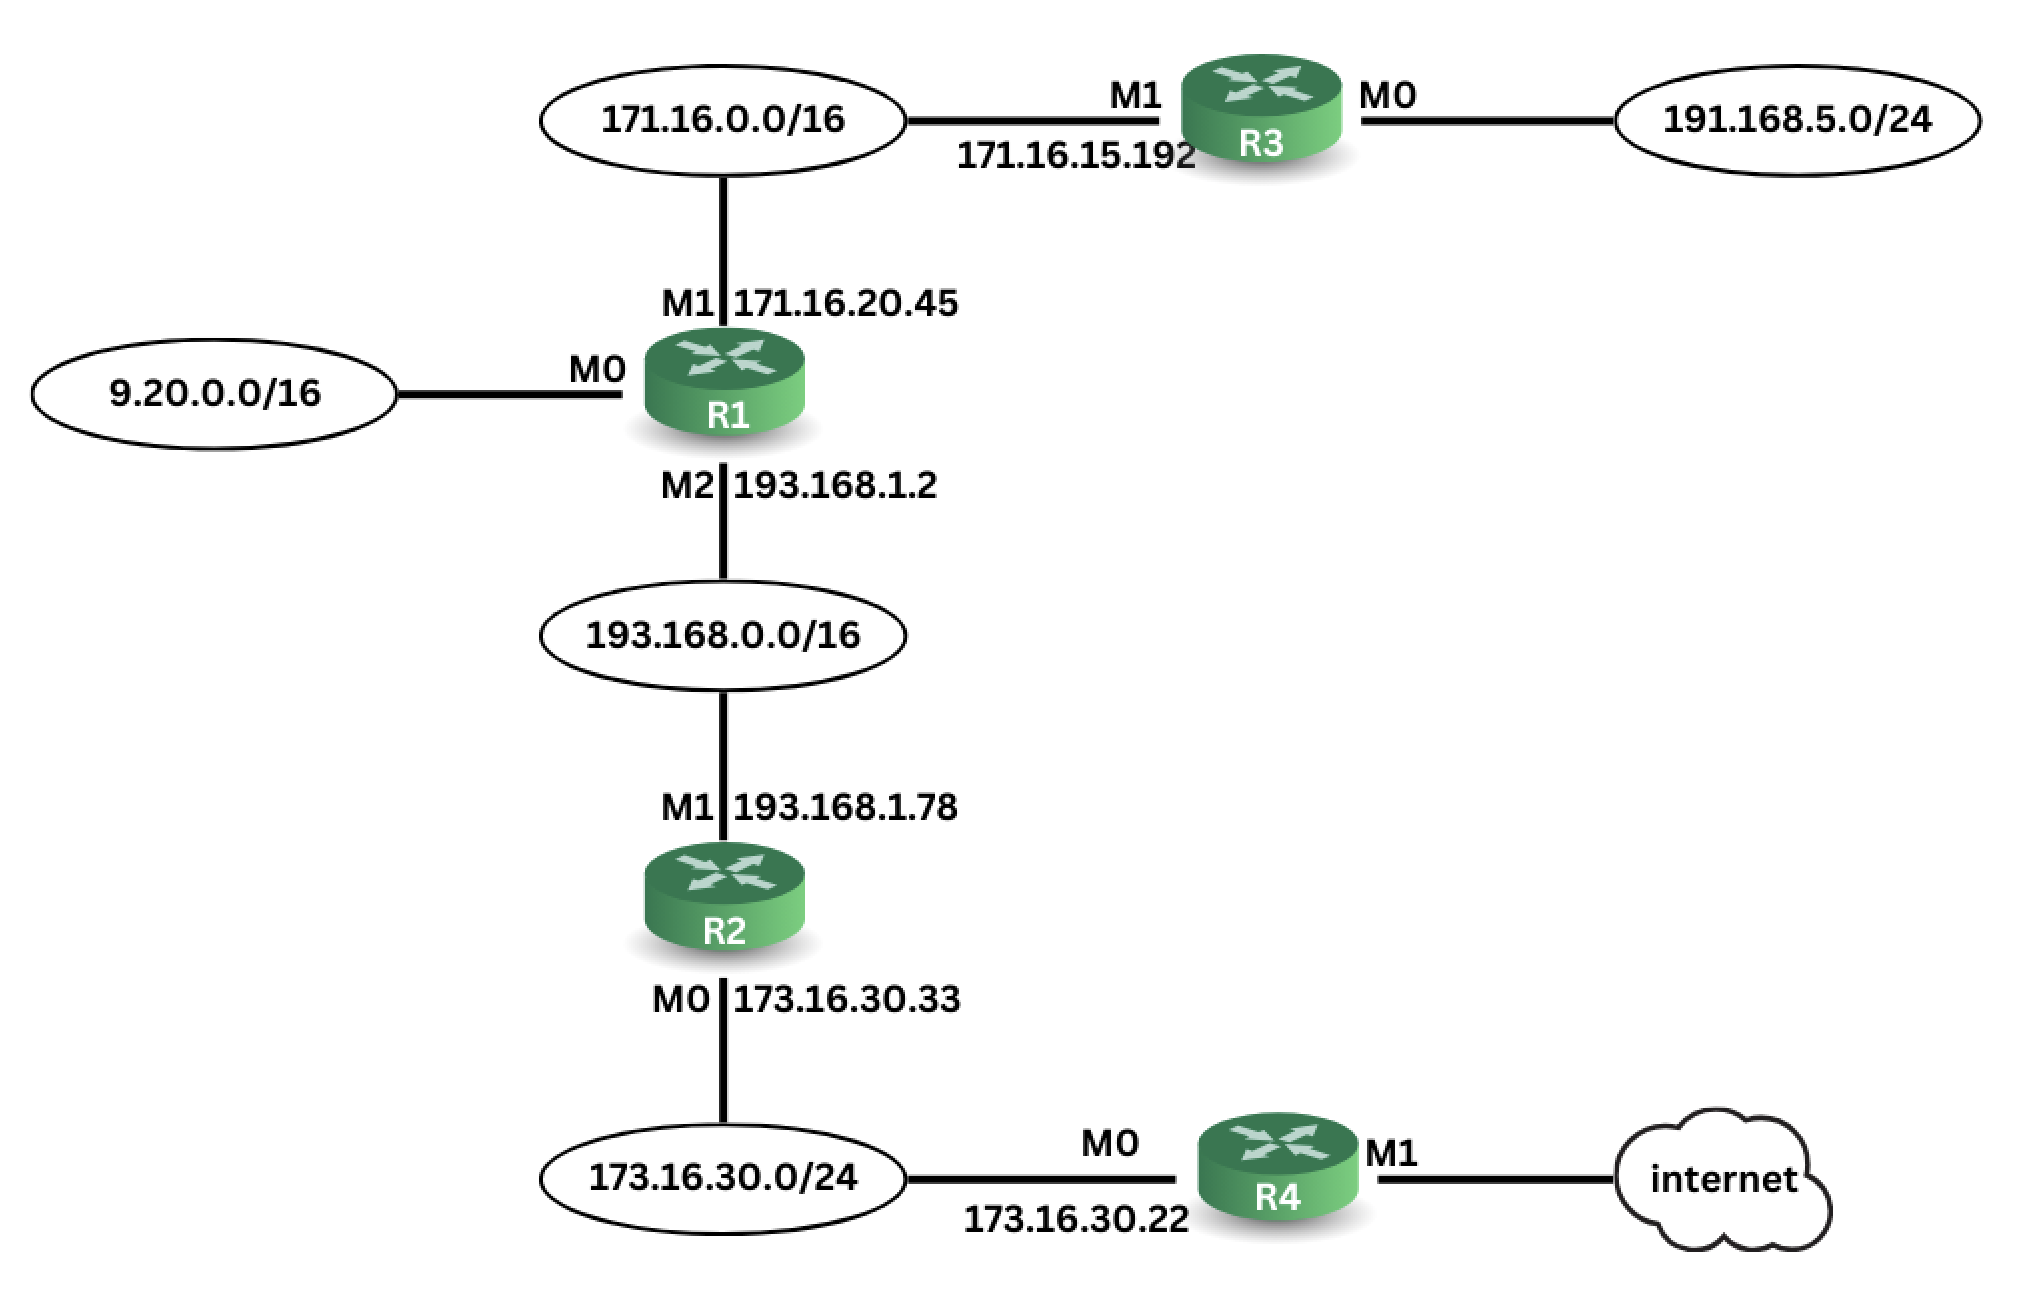
\includegraphics[width=0.8\textwidth]{question11.png}
    \begin{minipage}{0.8\textwidth}
        \centering
        Network configuration
    \end{minipage}
  \end{figure}

  \item Consider the network configuration of problem 11. Show the forwarding process if a packet
  \begin{enumerate}
    \item with the destination address 193.168.3.120 arrives at router R1

    /24 mask is applied, that results: 193.168.3.0. The network address doesn't exists in the table.

    /16 mask is applied, that results: 193.168.0.0. The network address does exists in the table.
    R1 router delivers the packet with the next hop address 193.168.3.120 through interface M2.

    \item with the destination address 174.16.30.144 arrives at router R2

    /24 mask is applied, that results: 174.16.30.0. The network address doesn't exists in the table.

    /16 mask is applied, that results: 174.16.0.0. The network address doesn't exists in the table.

    So R2 delivers the packet to the default router through interface M0 with next hop address 173.16.30.22.
  \end{enumerate}
  \item A network administrator uses the subnet mask 255.255.240.0 to configure the network 172.15.0.0.
  How many subnets have been created? How many usable addresses are there in each subnet? Assume classful addressing. (4 points)

  $240=1111000_2$. The prefix is therefore 8+8+4=/20.

  The address range is: 172.15.0.0/20-172.15.223.255.

  The number of addresses in this subnetwork is $2^{32-20}=2^12=4096$.
  The first and the last addresses are reserved for network address and broadcast addresses.
  So the number of usable addresses is 4094.

  \item Find the 1532nd address and the last address of the block 192.168.16.0/20. (4 points)

  1532/256=6. Since it is 0-indexed, 6.0-1=5.255.
  192.168.21.255

  \item An organization has been allocated a block of IP addresses.
  The IP address 154.101.43.163 is the 36th address in this block.
  The organization needs 72 IP addresses for hosts and routers. (4 points)
  \begin{enumerate}
    \item Specify the range of IP addresses that have been allocated to this organization.

    The first address is 154.101.43.163-35=154.101.43.128.
    
    To fit 72 addresses, the organization should be allocated 128 address. The mask should be $32-log(128)=32-7=25$.

    The last address should be: 154.101.43.128+127=154.101.43.255.

    So the range is: 154.101.43.128/25 to 154.101.43.255/25.
    
    \item Is there any wastage in this allocation? If so, calculate the number of IP addresses that are unused.

    The number of addresses not used is: 128-72-2=54.

    72 used for the organization, 1 used for network address and 1 for broadcast address.
  \end{enumerate}

  \item For each of the following destination IP addresses, determine which interface the router would use to forward the packet. Explain each answer. (5 points)
  \begin{enumerate}
    \item 187.123.224.131

    /25 mask is applied, that results: 187.123.224.128. The network address doesn't exists in the table.

    /18 mask is applied, that results: 187.123.192.0. The network address doesn't exists in the table.

    /17 mask is applied, that results: 187.123.128.0. The network address doesn't exists in the table.

    /15 mask is applied, that results: 187.122.0.0. The network address doesn't exists in the table.

    So the router forwards the packet to the default router through interface M4.
    
    \item 172.15.45.12

    /25 mask is applied, that results: 172.15.45.0. The network address doesn't exists in the table.

    /18 mask is applied, that results: 172.15.0.0. The network address doesn't exists in the table.

    /17 mask is applied, that results: 172.15.0.0. The network address doesn't exists in the table.

    /15 mask is applied, that results: 172.14.0.0. The network address doesn't exists in the table.

    So the router forwards the packet to the default router through interface M4.

    \item 201.4.200.20

    /25 mask is applied, that results: 201.4.200.0. The network address doesn't exists in the table.

    /18 mask is applied, that results: 201.4.192.0. The network address doesn't exists in the table.

    /17 mask is applied, that results: 201.4.128.0. The network address does exists in the table.

    So the router forwards the packet through interface M2.
    
    \item 187.123.224.50

    /25 mask is applied, that results: 187.123.224.0. The network address does exists in the table.

    So the router forwards the packet through interface M0.

    \item 180.75.20.10

    /25 mask is applied, that results: 180.75.20.0. The network address doesn't exists in the table.

    /18 mask is applied, that results: 180.75.0.0. The network address doesn't exists in the table.

    /17 mask is applied, that results: 180.75.0.0. The network address doesn't exists in the table.

    /15 mask is applied, that results: 180.74.0.0. The network address does exists in the table.

    So the router forwards the packet through interface M3.

  \end{enumerate}
\end{enumerate}


\end{document}